\newpage

\subsection{Effective implementation}

\textbf{Methodologies:} Practical experiments, prototyping

Before implementing real-time in a web application it is important to make a suitable decision if you want to use WebSockets or Server Sent-Events. This comes down to choosing between bidirectional or unidirectional communication.

A feature can be implemented in real-time using two different approaches. The first approach utilizes WebSockets, where data is sent from the client to the server through a bidirectional connection. Subsequently, the server sends the updated data to other clients, maintaining a continuous, interactive communication channel. The second approach leverages HTTP requests for data transmission from the client to the server. The server then updates the clients using Server-Sent Events (SSE), which only requires a unidirectional persistent connection. This method simplifies the communication model by using HTTP for sending data and SSE for receiving updates.

This means there is a difference between needing bidirectional communication and choosing to use it. In some use cases choosing for a HTTP request to send data is not sufficient enough and can impact the performance:

\begin{enumerate}
  \item Canvas tools: Figma, Miro
  \item Multiplayer games
  \item Text-editing
\end{enumerate}

The data that needs to be constantly transmitted can benefit from a bidirectional connection because the connection is persistent and doesn't have to be established for each change. However, for other features, this level of persistence is unnecessary, and an HTTP request is sufficient. For example

\begin{enumerate}
  \item Live status boards
  \item Form submissions
  \item Notifications
\end{enumerate}

Lastly it is important to think about how to ensure the application is future-proof. Choosing SSE limits options for future bidirectional communication features, while starting with WebSockets avoids this issue. This trade-off is crucial. 

\subsubsection{WebSockets implementation}

To illustrate the practical use of WebSockets, a proof of concept (POC) will be developed to understand the two types of features. Feature 1 utilizes WebSockets in a scenario where Server-Sent Events (SSE) would suffice, while feature 2 requires bidirectional communication. The first feature will be a status board, and the second will be a canvas with moving objects. Socket.io is chosen for this demonstration due to its ease of implementation and rich feature set, showcasing the advantages a robust library can offer.

\textbf{POC setup}

\begin{figure}[h]
  \caption{POC diagram}
  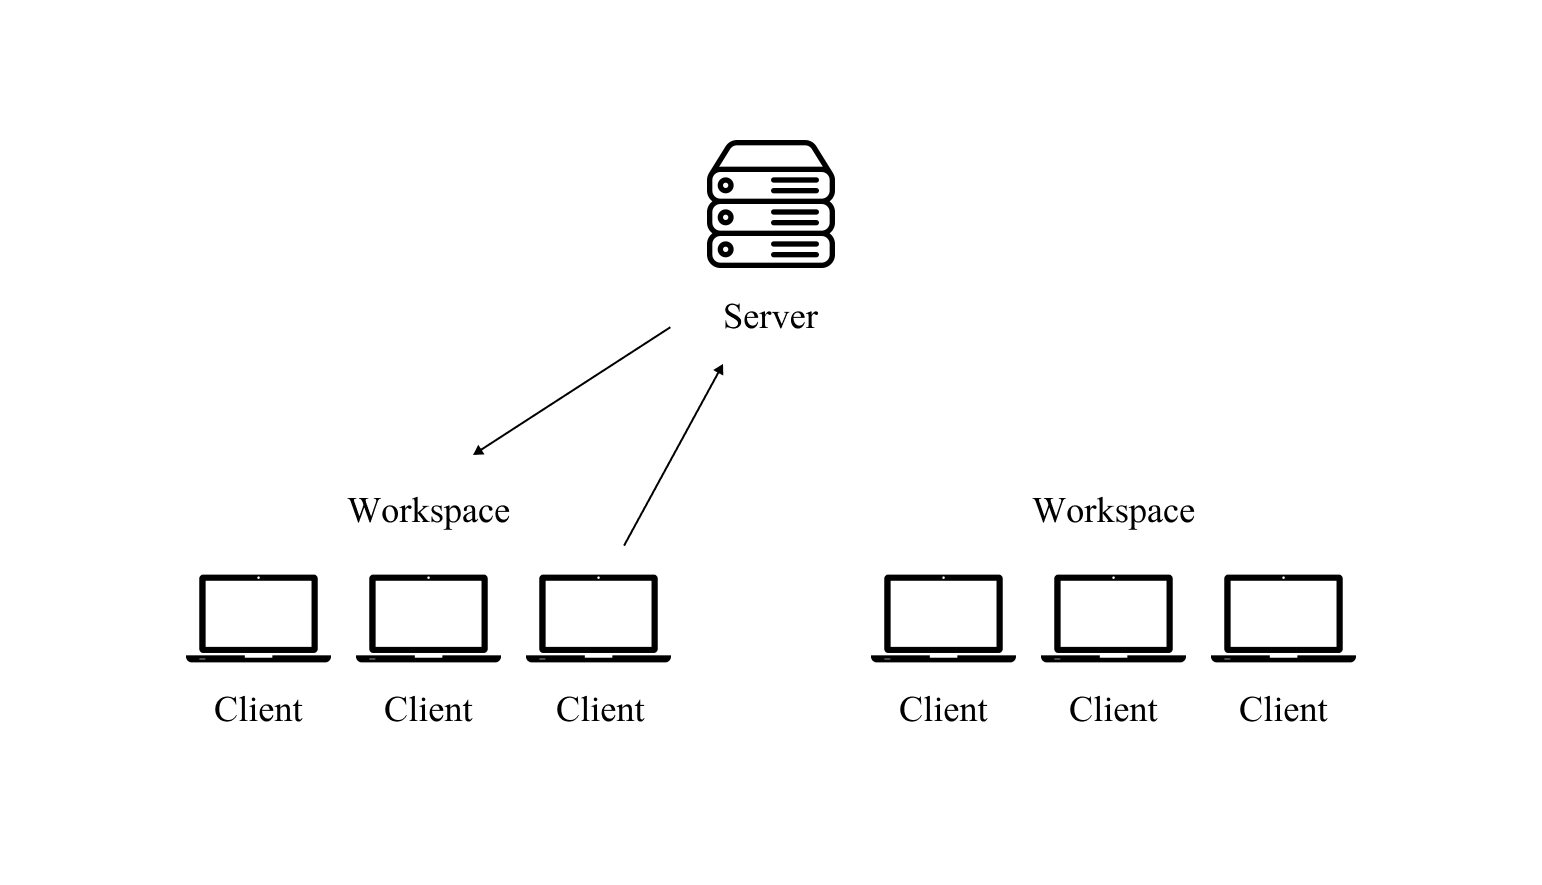
\includegraphics[width=0.80\linewidth]{POC_diagram}
  \centering
\end{figure}

Before delving into feature implementation within this POC, certain prerequisites must be addressed. Collaboration entails multiple users working together, necessitating robust user authentication and authorization mechanisms.

The server in this POC will be created with Express and TypeScript because of the straightforward implementation. Other dependencies include JWT for token-based authentication, bcrypt for password hashing and Prisma as ORM. Prisma is a tool that provides an easy way of setting up a data schema.

\begin{lstlisting}[caption=Prisma Data Schema]
  model User {
    name      String      @id @unique
    password  String
    workspace Workspace[]
  }

  model Workspace {
    name  String @id @unique
    users User[]
    board Task[]
  }
  ...
\end{lstlisting}

After login and register HTTP routes to our server an authMiddleware is added to finalise the authentication. These users now need a way of defining how to collaborate. In collaborative features end users don't just work with anybody, they choose who has access to their workspace. The final step of the setup is providing the users with these workspaces which can already be seen in the schema, see Listing 5.

\begin{lstlisting}[caption=WorkspaceController]
  export class WorkspaceController {
    static async list(req: AuthenticatedRequest, res: Response) {
      const user = req.user;
   
      try {
        const workspaces = await WorkspaceService.list(user);
        res.status(200).json(workspaces);
      } catch (error: any) {
        res.status(400).json({ error: error.message });
      }
    }
   
    static async get(req: AuthenticatedRequest, res: Response) {
      const { name } = req.params;
      const user = req.user;
   
      try {
        const workspace = await WorkspaceService.get(name, user);
        res.status(200).json(workspace);
      } catch (error: any) {
        res.status(400).json({ error: error.message });
      }
    }
    // ...
  }   
\end{lstlisting}

\textbf{Feature 1: Task status board}

The initial step involves setting up the server using Socket.IO, which can utilize the same host as the existing HTTP endpoints. This integration is possible because the WebSocket connection handshake leverages HTTP for establishment, see 2.1.4 WebSocket fundamentals. Upon each incoming socket connection to the server, the 'connection' event is triggered, creating a socket bound to a specific client. This socket enables listening to the client's individual incoming events. Given that not all users need to receive events from every other user but only from those within the same workspace, Socket.IO offers a feature enabling sockets (clients) to join a certain room. Then the server can selectively relay incoming client data only to other users within the same room (workspace) \cite{socketio}. This capability showcases what Socket.IO brings to the table, while not complex to implement, it offers convenient out-of-the-box functionality.

Using the socket it is easy to define all incoming events in a scalable way. Creating a task and updating a task must be sent to the other clients.

\begin{lstlisting}[caption=WebSocket connection event handler]
  export default function eventHandler(io: Server) {
    io.on("connection", (socket: Socket) => {
      const { workspace, type } = socket.handshake.query;
      const room = type ? `${workspace}-${type}` : workspace;
      socket.join(room as string);
      console.log(`Client connected to workspace: ${room}`);
   
      createTaskHandler(socket as AuthenticatedSocket, io);
      updateTaskHandler(socket as AuthenticatedSocket, io);
   
      socket.on("disconnect", () => {
        console.log("Client disconnected");
      });
    });
  }
\end{lstlisting}

\begin{lstlisting}[caption=WebSocket task events handlers]
  export const createTaskHandler = async (
    socket: AuthenticatedSocket,
    io: Server
   ) => {
    socket.on("createTask", async (data) => {
      try {
        const { title, status, workspace } = data;
   
        const task = await TaskService.create(title, status, workspace);
   
        io.to(workspace).emit("taskCreated", task);
      } catch (error: any) {
        socket.emit("taskError", { error: error.message });
      }
    });
   };
   
   export const updateTaskHandler = async (
    socket: AuthenticatedSocket,
    io: Server
   ) => {
    socket.on("updateTask", async (data) => {
      try {
        const { taskId, status, workspace } = data;
   
        const task = await TaskService.update(taskId, status, workspace);
   
        io.to(workspace).emit("taskUpdated", task);
      } catch (error: any) {
        socket.emit("taskError", { error: error.message });
      }
    });
  };
\end{lstlisting}

It's crucial to highlight that the WebSocket connection undergoes authentication using the same token. Socket.IO seamlessly facilitates passing this token during the handshake \cite{socketio}. This becomes particularly advantageous considering that the native WebSocket API lacks support for passing authentication headers. Alternatives, such as transmitting the token via query parameters pose security risks. Notably, authorization considerations were omitted in this proof of concept (POC), as security isn't a concern within the scope. While authorization implementation isn't inherently complex, it's deemed time-intensive and thus ignored in future iterations.

\begin{lstlisting}[caption=Auth Middleware for the socket]
  export const authenticateSocket = async (socket: Socket, next: any) => {
    try {
      const token = socket.handshake.auth.token;
      if (!token) throw new Error("No token provided");
   
      const jwtSecret = process.env.JWT_SECRET as string;
      if (!jwtSecret) throw new Error("JWT_SECRET not set");
   
      const user = jsonwebtoken.verify(token, jwtSecret) as JwtPayload;
      if (!user) throw new Error("User not found in token");
   
      (socket as AuthenticatedSocket).username = user.name;
      next();
    } catch (error: any) {
      next(error);
    }
  };
\end{lstlisting}

Now, it's time to integrate the client side to establish the real time task status board. Following the setup of basic pages facilitating user authentication, registration, workspace creation, and user invitation via HTTP endpoints, the WebSocket functionality can be introduced. For this proof of concept (POC), the JavaScript framework React, coupled with TypeScript, will be utilized, given its adoption within Teamleader and the extensive community backing.

Socket.IO offers a client library designed to seamlessly connect to the WebSocket server. Leveraging this library simplifies the process of passing the authentication token during the handshake.

\begin{lstlisting}[caption=Using the WebSocket]
  export default function Board() {
    const navigate = useNavigate();
    const { username, token } = useAuthentication();
    const { name } = useParams();
    const [socket, setSocket] = useState<Socket>();
    const [newTask, setNewTask] = useState("");
    const [tasks, setTasks] = useState<Task[]>([]);
   
    useEffect(() => {
      const newSocket = io("http://localhost:3000", {
        auth: { token },
        query: { workspace: name },
      });
      setSocket(newSocket);
   
      return () => {
        newSocket.close();
      };
    }, [name, token]);
    // ... 
  }  
\end{lstlisting}

Since the sockets exclusively transmit new or updated tasks, the initial loading of persisted data must occur upon initialization. This scenario presents an ideal use case for a GET request, eliminating the necessity for WebSocket involvement. During page rendering, persisted data will be loaded.

Alternatively, an additional approach worth considering involves sending the initial data over the socket connection. While an HTTP GET request perfectly suits this purpose, leveraging sockets for this task remains feasible, particularly considering their existing utilization within the application.


\begin{lstlisting}[caption=Loading persisted data]
  useEffect(() => {
    async function fetchTasks() {
      const response = await TaskService.getAll(name as string);
      const data = await response.json();
 
      if (response.ok) {
        setTasks(data);
      } else if (response.status === 401) {
        navigate("/login");
      } else {
        console.error(data.error);
      }
    }
 
    fetchTasks();
  }, [name, navigate]);
\end{lstlisting}

The initial data is set and the WebSocket connection is alive, the next steps consist of listening to events: new task and updated task, and also emitting those events to the server.

\begin{lstlisting}[caption=Listening to events]
  useEffect(() => {
    if (socket) {
      socket.on("taskCreated", (task) => {
        setTasks([...tasks, task]);
      });
 
      socket.on("taskUpdated", (task) => {
        setTasks((prevTasks) =>
          prevTasks.map((t) => (t.id === task.id ? task : t))
        );
      });
 
      socket.on("taskError", (data) => {
        console.error(data.error);
      });
 
      socket.on("connect_error", (error) => {
        console.error(error);
      });
    }
  }, [socket, tasks]);
\end{lstlisting}

\begin{lstlisting}[caption=Sending events]
  const handleSubmitTask = (event: React.FormEvent<HTMLFormElement>) => {
    event.preventDefault();
    if (!socket) return;
    socket.emit("createTask", {
      title: newTask,
      status: "to do",
      workspace: name,
    });
    setNewTask("");
  };
 
  const updateTaskStatus = async (taskId: number, status: string) => {
    if (!socket) return;
    socket.emit("updateTask", {
      taskId,
      status,
      workspace: name,
    });
  };
\end{lstlisting}

\textbf{Synchronization}

One of the primary challenges encountered when developing this POC is the potential for data desynchronization in real-time interactions. Indeed, it is possible that data alterations may occur while the client awaits the arrival of initial requests. Addressing this issue necessitates implementing server-side logic to manage synchronization requests from clients. However, a more proactive approach involves ensuring data integrity from the start, thereby preemptively reducing desynchronization concerns.

One potential solution involves initiating the connection prior to HTTP fetching, thus preempting the possibility of initial data overriding client-side data. Instead, newly arrived data would be added to existing client data, ensuring synchronization. Given the complexity of addressing synchronization challenges in this POC, it would be beneficial to draw insights from the case study of Figma, see Appendix A.

\textbf{Feature 2: Design canvas}

All multiplayer design canvas apps have one feature in common, live cursor sharing. This feature perfectly demonstrates the need for a persistent connection when sending data to the server. Implementing it also starts by adding a new event listener to the WebSocket server.

\begin{lstlisting}[caption=Cursor Event Handler]
export const cursorHandler = (socket: AuthenticatedSocket, io: Server) => {
  socket.on("mousePosition", (data) => {
    try {
      const { username, position, room } = data;

      io.to(room).emit("mousePosition", { username, position });
    } catch (error: any) {
      socket.emit("cursorError", { error: error.message });
    }
  });
};
\end{lstlisting}

Upon receiving this event, the server sends the data to every other user linked to the same room. It's noteworthy that the persistence of this data is unnecessary. However, when incorporating real-time objects onto the canvas necessitating persistence, synchronization complexities emerge, as elaborated in Appendix A.

On the client side, each connected user transmits their cursor location through this event. Simultaneously, the clients are listening to the event to display the real-time positions of all other users' cursors.

\begin{lstlisting}[caption=Client sending cursor data to server]
    const handleMouseEnter = (event: MouseEvent) => {
      if (!socket || !canvasRef.current) return;
      const canvasRect = canvasRef.current.getBoundingClientRect();
      const mouseX = event.clientX - canvasRect.left;
      const mouseY = event.clientY - canvasRect.top;
    
      const userPosition = {
        username,
        position: {
          x: mouseX,
          y: mouseY,
        },
        room: `${name}-design`,
      };
      socket.emit("mousePosition", userPosition);
    };
    
    canvas.addEventListener("mousemove", handleMouseEnter);
\end{lstlisting}

\begin{lstlisting}[caption=Client receiving other cursor data]
  socket.on("mousePosition", (userPosition) => {
    setUserPositions((prevPositions) => {
      return {
        ...prevPositions,
        [userPosition.username]: userPosition.position,
      };
    });
  });
\end{lstlisting}

Finally, this positional data is rendered onto the canvas. An important insight learned from crafting this feature is whether it is necessary to have consistently perfect real-time synchronization. The answer is in fact that it is not necessary. While real-time functionality is essential, it is acceptable to introduce a slight buffer when transmitting cursor positions to the server. By implementing e.g. a 100ms buffer, the server's workload is significantly reduced. Admittedly, this approach may induce flickering on the client side upon receiving these location updates. Nevertheless, this issue can be readily addressed by implementing smooth transitions between each position update.

\subsubsection{Server-Sent Events implementation}

Features that can benefit from unidirectional communication, specifically from server to client, are achievable through WebSocket connections. However, opting for Server-Sent Events offers a simpler approach. Two implementation approaches are up for discussion: firstly, a client sends data to the server via HTTP POST, which the server then broadcasts to other clients; secondly, the server initiates an event to the clients, prompting them to make a new GET request. While the first method obtains less overhead, the second approach proves to be more robust. Requesting clients to fetch again ensures a sync issue-free environment without any extra implementations. Nevertheless, the first method essentially represents a less efficient WebSocket implementation. Developers benefit from embracing WebSockets from the start, particularly for future-proofing feature expansions that demand bidirectional communication. Conversely, the second approach aligns seamlessly with scenarios involving the transition of non-real-time functionalities into real-time capabilities or the implementation of basic notifications.

\textbf{Converting into real-time}

Within the POC there are some places not in real-time because they use normal HTTP requests. For example, the homepage shows every workspace an end user is part of but when a user is added to someone's workspace this is not shown in real-time, the user must refresh the webpage. A perfect situation to convert something that is not in real-time to be in real-time since in a lot of projects it doesn't make sense to start rewriting the backend.

The idea behind SSE is to keep the HTTP connection alive and transmit data over that connection \cite{w3-sse}. To emit data from places in the server code EventEmitter is used, something built into Node.js.

\begin{lstlisting}[caption=]
  router.get("/sse", (req, res) => {
    const username = req.query.username as string;
   
    res.setHeader("Content-Type", "text/event-stream");
    res.setHeader("Cache-Control", "no-cache");
    res.setHeader("Connection", "keep-alive");
   
    eventEmitter.on(`invite:${username}`, (data) =>
      res.write(`event: invite:${username}\ndata: ${JSON.stringify(data)}\n\n`)
    );
   
    res.on("close", () => {
      eventEmitter.off(`test`, (data) => res.write(data));
    });
  });
\end{lstlisting}

The connection is left alive by setting the connection to keep-alive in the header. Content type is set to even-stream so data can be streamed over the connection. Lastly, the data sent to the client needs to be in a certain format to define it as SSE \cite{html-spec-sse}:

Event: eventname\\
data: "string"

Now this EventEmitter instance can be used when a client calls the invite endpoint.

\begin{lstlisting}[caption=]
  static async invite(
    req: AuthenticatedRequest,
    res: Response,
    eventEmitter: any
  ) {
    const { name } = req.params;
    const { username } = req.body;
    const user = req.user;
 
    try {
      await WorkspaceService.invite(name, username, user);
      eventEmitter.emit(`invite:${username}`, { workspace: name });
      res.status(200).send();
    } catch (error: any) {
      res.status(400).json({ error: error.message });
    }
  }
\end{lstlisting}

After this setup, the client can use the EventSource API and add EventListeners to those custom event names \cite{w3-sse}.

\begin{lstlisting}[caption=]
  useEffect(() => {
    if (username) {
      const eventSource = new EventSource(
        "http://localhost:3000/sse?username=" + username
      );
 
      eventSource.addEventListener(`invite:${username}`, (event) => {
        setWorkspaces((workspaces) => [
          ...workspaces,
          { name: JSON.parse(event.data).workspace },
        ]);
      });
    }
  }, [username]);
\end{lstlisting}

It's crucial to acknowledge that native Server-Sent Events (SSE) lack support for passing headers, similar to native WebSocket. Because this POC is already set up with token-based authentication, changing to cookie-based authentication is not an ideal solution. Instead passing the token as a query parameter is possible but not ideal.

However, it's worth noting that Mercure, as a powerful open-source tool, addresses these authentication limitations by providing robust support for token-based authentication. 

\textbf{Notifications with Mercure}

Finally, Mercure is a solution where the developer doesn't have to deal with any of the real-time server side. This setup is very straightforward. The Mercure Hub server can be created with a simple docker compose \cite{mercure}. 

\begin{lstlisting}[caption=docker-compose.yaml for Mercure Hub]
services:
  mercure:
    image: dunglas/mercure
    restart: unless-stopped
    environment:
      SERVER_NAME: ":80"
      MERCURE_PUBLISHER_JWT_KEY: "!ChangeThisMercureHubJWTSecretKey!"
      MERCURE_SUBSCRIBER_JWT_KEY: "!ChangeThisMercureHubJWTSecretKey!"
      MERCURE_EXTRA_DIRECTIVES: "cors_origins http://localhost:5173"
    command: /usr/bin/caddy run --config /etc/caddy/Caddyfile.dev
    healthcheck:
      test: ["CMD", "curl", "-f", "https://localhost/healthz"]
      timeout: 5s
      retries: 5
      start_period: 60s
    ports:
      - "80:80"
      - "443:443"
    volumes:
      - mercure_data:/data
      - mercure_config:/config

volumes:
  mercure_data:
  mercure_config:
\end{lstlisting}

Now the server can send POST requests to this hub whenever it wants to. In the following example when a task is created this gets communicated the Mercure Hub using axios to send a POST request.

\begin{lstlisting}[caption=POST request to the Mercure Hub]
export const publishNotification = async (topic: string, data: any) => {
  try {
    await axios.post(
      MERCURE_HUB_URL as string,
      {
        data: data,
        topic: topic,
      },
      {
        headers: {
          "Content-Type": "application/x-www-form-urlencoded",
          Authorization: `Bearer ${process.env.MERCURE_JWT_TOKEN}`,
        },
      }
    );
  } catch (error) {
    console.error("Failed to publish notification:", error);
  }
};
\end{lstlisting}

\begin{lstlisting}[caption=]
export default class TaskService {
  static async create(title: string, status: string, workspacename: string) {
    try {
      const task = await prisma.task.create({
        data: {
          title,
          status,
          board: {
            connect: {
              name: workspacename,
            },
          },
        },
      });

      await publishNotification(title, `workspace/${workspacename}/task`);

      return task;
    } catch (error: any) {
      throw new Error(error);
    }
  }
  ...
\end{lstlisting}

Now the client can listen to the Mercure Hub using Server-Sent Events. Because notifications are across the entire app it makes sense to write a provider with a context.

\begin{lstlisting}[caption=EventSource listening to the topic]
  useEffect(() => {
    const fullUrl = config.mercureUrl + topic;

    const eventSource = new EventSource(fullUrl);

    eventSource.onmessage = (event) => {
      const newData = JSON.parse(event.data);
      setData(newData);
    };

    eventSource.onerror = (error) => {
      console.error("Failed to connect to Mercure:", error);
    };

    return () => {
      eventSource.close();
    };
  }, [topic]);
\end{lstlisting}

\subsubsection{AsyncAPI Specification}

AsyncAPI is an open-source initiative and specification designed to provide a standardized way to define and document event-driven APIs. Similar to how OpenAPI (formerly known as Swagger) standardizes RESTful APIs, AsyncAPI aims to bring a similar level of standardization and clarity to the world of event-driven and message-driven architectures. \cite{asyncapi}

In the context of WebSockets, AsyncAPI provides a standardized way to describe the communication channels and message exchanges that occur over a WebSocket connection. This can include defining the various events or messages that a client can send to a server and vice versa, along with the structure of these messages.

\textbf{Key features}

\begin{enumerate}
  \item Standardized Documentation
  \item Schema Definitions
  \item Protocol-Specific Features
  \item Interactive Documentation
  \item Code Generation
\end{enumerate}

Consider an example of a WebSocket-based chat application. The following AsyncAPI document describes the API for such an application, where clients can send messages to a chat room and receive messages from other participants. \cite{asyncapi-docs}

\begin{lstlisting}[caption=EventSource listening to the topic]
asyncapi: 3.0.0
info:
  title: Chat Application API
  version: 1.0.0
  description: Example of a WebSocket chat application

channels:
  chatMessage:
    address: /chatMessage
    messages:
      chatMessage:
        $ref: '#/components/messages/chatMessage'
  chatReply:
    address: /chatReply
    messages:
      chatReply:
        $ref: '#/components/messages/chatReply'

operations:
  sendMessage:
    action: send
    channel:
      $ref: '#/channels/chatMessage'
    reply:
      channel:
        $ref: '#/channels/chatReply'

components:
  messages:
    chatMessage:
      payload:
        type: object
        properties:
          user:
            type: string
          message:
            type: string
    chatReply:
      payload:
        type: object
        properties:
          user:
            type: string
          message:
            type: string
          timestamp:
            type: string
            format: date-time
\end{lstlisting}

AsyncAPI is a powerful tool for documenting and managing WebSocket-based APIs. By providing a standardized way to describe WebSocket communication channels and message formats, AsyncAPI improves collaboration, reduces integration errors, and accelerates development.

\subsubsection{Conclusion}

In conclusion, implementing real-time features in a web application requires careful consideration of the communication method, whether it be WebSockets for bidirectional communication or Server-Sent Events (SSE) for unidirectional communication. WebSockets are ideal for applications needing constant, interactive exchanges between clients and servers, such as canvas tools, multiplayer games, and collaborative text editors. On the other hand, SSE is suitable for simpler scenarios like live status boards, real-time statistics, and notifications where bidirectional communication is unnecessary.

Future-proofing the application is crucial; starting with WebSockets provides flexibility for later expansion into features requiring bidirectional communication. This trade-off needs to be considered at the design phase to avoid complexities in future updates.

The Proof of Concept (POC) \cite{poc-client} \cite{poc-server} showcased the effective use of WebSockets and SSE, demonstrating their implementation for a task status board and a design canvas, respectively. WebSockets facilitated real-time updates and interactions, while SSE provided a simpler, efficient method for streaming updates to clients without the need for a persistent connection. Additionally, tools like Mercure enhance SSE by offering robust support for token-based authentication and simplifying server-side setup.

Finally, adopting AsyncAPI specifications can standardize documentation and implementation of event-driven APIs, ensuring clarity and interoperability across different components of a real-time web application. By considering these factors and leveraging appropriate technologies, developers can effectively implement and maintain real-time features in their web applications.
